\documentclass[letterpaper,12pt]{article}
\usepackage{array}
\usepackage{threeparttable}
\usepackage{geometry}
\geometry{letterpaper,tmargin=1in,bmargin=1in,lmargin=1.25in,rmargin=1.25in}
\usepackage{fancyhdr,lastpage}
\pagestyle{fancy}
\lhead{}
\chead{}
\rhead{}
\lfoot{\footnotesize\textsl{OSM Lab, Summer 2017, Math PS \#6}}
\cfoot{}
\rfoot{\footnotesize\textsl{Page \thepage\ of \pageref{LastPage}}}
\renewcommand\headrulewidth{0pt}
\renewcommand\footrulewidth{0pt}
\usepackage[format=hang,font=normalsize,labelfont=bf]{caption}
\usepackage{amsmath}
\usepackage{amssymb}
\usepackage{amsthm}
\usepackage{natbib}
\usepackage{setspace}
\usepackage{float,color}
\usepackage[pdftex]{graphicx}
\usepackage{hyperref}
\hypersetup{colorlinks,linkcolor=red,urlcolor=blue,citecolor=red}
\theoremstyle{definition}
\newtheorem{theorem}{Theorem}
\newtheorem{acknowledgement}[theorem]{Acknowledgement}
\newtheorem{algorithm}[theorem]{Algorithm}
\newtheorem{axiom}[theorem]{Axiom}
\newtheorem{case}[theorem]{Case}
\newtheorem{claim}[theorem]{Claim}
\newtheorem{conclusion}[theorem]{Conclusion}
\newtheorem{condition}[theorem]{Condition}
\newtheorem{conjecture}[theorem]{Conjecture}
\newtheorem{corollary}[theorem]{Corollary}
\newtheorem{criterion}[theorem]{Criterion}
\newtheorem{definition}[theorem]{Definition}
\newtheorem{derivation}{Derivation} % Number derivations on their own
\newtheorem{example}[theorem]{Example}
\newtheorem{exercise}[theorem]{Exercise}
\newtheorem{lemma}[theorem]{Lemma}
\newtheorem{notation}[theorem]{Notation}
\newtheorem{problem}[theorem]{Problem}
\newtheorem{proposition}{Proposition} % Number propositions on their own
\newtheorem{remark}[theorem]{Remark}
\newtheorem{solution}[theorem]{Solution}
\newtheorem{summary}[theorem]{Summary}
%\numberwithin{equation}{section}
\bibliographystyle{aer}
\newcommand\ve{\varepsilon}
\newcommand\boldline{\arrayrulewidth{1pt}\hline}

\usepackage{graphicx}
\DeclareGraphicsExtensions{.pdf,.png,.jpg,.gif}


\begin{document}

\begin{flushleft}
   \textbf{\large{Math Homework Week \#6, Linear Contrained Optimization}} \\[5pt]
   OSM Lab, Eun-Seok Lee \\[5pt]

\end{flushleft}

\vspace{5mm}

\begin{enumerate}



	\item (8.1) \\
\begin{figure}[htbp]
\begin{center}
    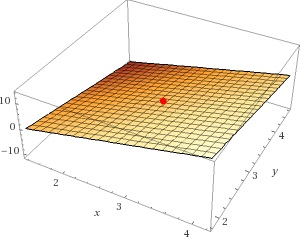
\includegraphics[scale=0.9]{8p1a}
    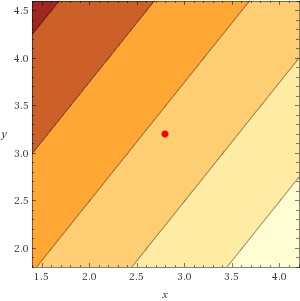
\includegraphics[scale=0.5]{8p1b}
    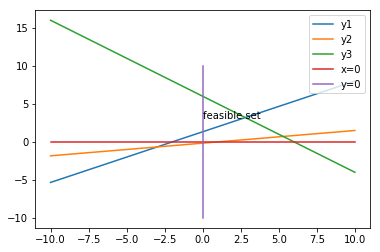
\includegraphics[scale=0.5]{8p1c}
    \caption{} \label{fig:label}
\end{center}
\end{figure}
	From vertices, $x = (14/5, 16/5)$ is optimizer.


	\item (8.2) \\
(i) \\
\begin{figure}[htbp]
\begin{center}
    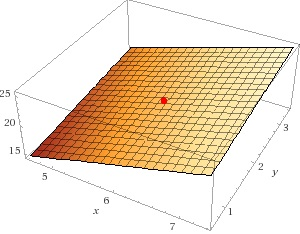
\includegraphics[scale=0.9]{8p2a}
    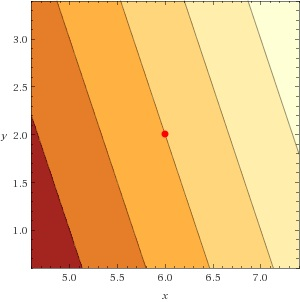
\includegraphics[scale=0.5]{8p2b}
    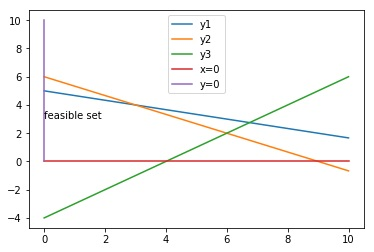
\includegraphics[scale=0.5]{8p2c}
    \caption{} \label{fig:label}
\end{center}
\end{figure}
From vertices, $x = (6, 2)$ is optimizer.\\ The optimal value is 20.\\ Figures are below.\\
\\
\\
\\
(ii) \\
\begin{figure}[htbp]
\begin{center}
    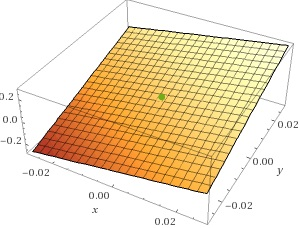
\includegraphics[scale=0.9]{8p2d}
    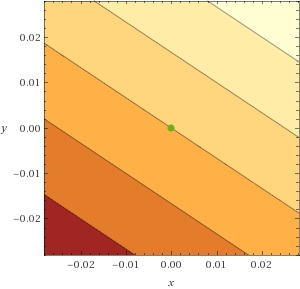
\includegraphics[scale=0.5]{8p2e}
    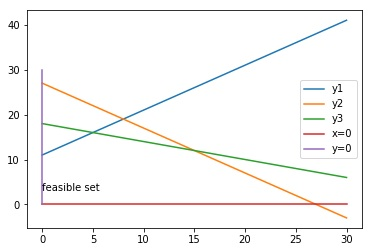
\includegraphics[scale=0.5]{8p2f}
    \caption{} \label{fig:label}
\end{center}
\end{figure}
From vertices, $(x, y) = (15, 12)$ is optimizer.\\ The optimal value is 132.\\ Figures are below.\\


	\item (8.5) \\
(i) "By Hand," \\
1) $f = 3x +y \\
w_1 = 15-x-3y\\
w_2 = 18 - 2x - 3y \\
w_3 = 4 - x + y\\$
\\
2) $f = 4y + 12 - 3w_3\\
w_1 = 11 - 2y + w_3\\
w_2 = 10 -5y +2w_3\\
x = 4 + y - w_3\\$
\\
3) $f = 4(2+\frac{2}{5}w_3-\frac{1}{5}w_2) + 12 -3w_3\\
w1 = 11 - 2(2+\frac{2}{5}w_3-\frac{1}{5}w_2) + w_3\\
y = (2+\frac{2}{5}w_3-\frac{1}{5}w_2)\\
x = 4 + (2+\frac{2}{5}w_3-\frac{1}{5}w_2) - w_3\\$
\\
The optimizer is (6, 2), and it is exactly same to (8.2).

(ii) I used the simplex solver, and its optimizer is (15, 12) and it is exactly same to (8.2). The dictionaries are below.
\begin{figure}[htbp]
\begin{center}
    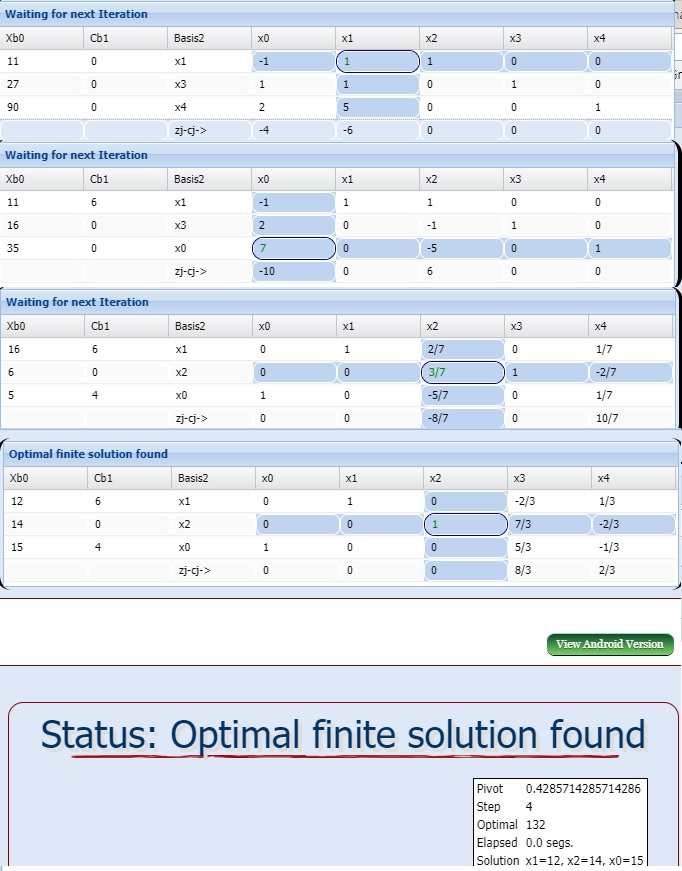
\includegraphics[scale=0.46]{8p5b}
    \caption{} \label{fig:label}
\end{center}
\end{figure}

	\item (8.7) \\
(i) The optimizer is (3, 4) and optimal value is 11.\\
(ii) It is NOT feasible.\\
(iii) The optimizer is (0, 2) and optimal value is 2.

Each dictionary is below.

\begin{figure}[htbp]
\begin{center}
    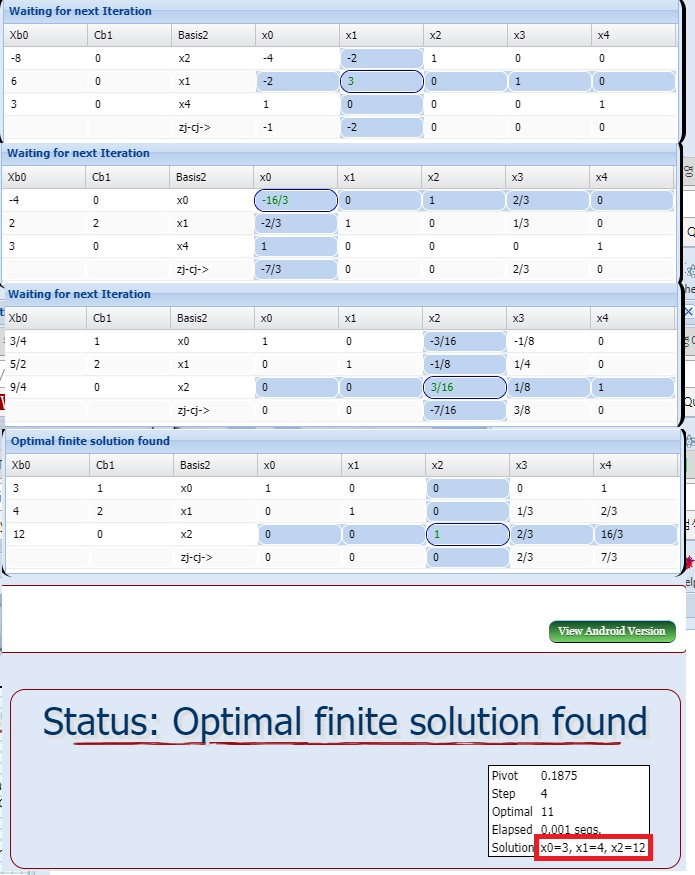
\includegraphics[scale=0.46]{8p7a}
    \caption{(i)} \label{fig:label}
\end{center}
\end{figure}

\begin{figure}[htbp]
\begin{center}
    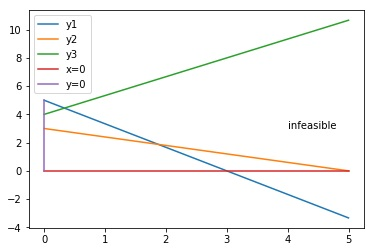
\includegraphics[scale=0.51]{8p7b}
    \caption{(ii)} \label{fig:label}
\end{center}
\end{figure}
'
\begin{figure}[htbp]
\begin{center}
    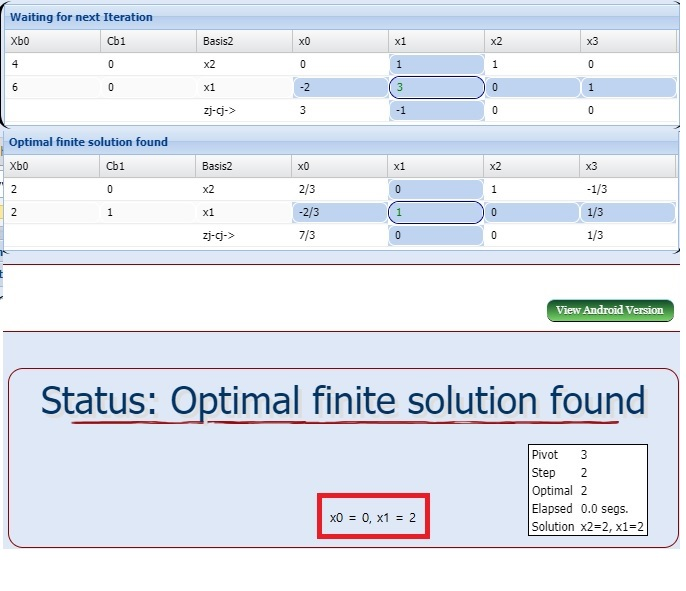
\includegraphics[scale=0.46]{8p7c}
    \caption{(iii)} \label{fig:label}
\end{center}
\end{figure}
\phantom{aaaaa}
\phantom{aaaaa}
\phantom{aaaaa}
\phantom{aaaaa}
\phantom{aaaaa}
\phantom{aaaaa}
\phantom{aaaaa}
\phantom{aaaaa}
\phantom{aaaaa}
\phantom{aaaaa}
\phantom{aaaaa}\\
\\
\\

	\item (8.13) \\
If each constraint is zero, it means that only feasible set is $(0, \cdots, 0)$.\\
If $c^Tx$ is defined at $x = (0, \cdots, 0)$, then it is optimum.\\
However, if it is not defined, it is unbounded by definition.


	\item (8.17) From dual problem, I will restore primal problem by definition.\\ \\
min $ b^Ty\\
s.t. A^Ty \geq c\\
y \geq 0$
\\ \\
By the definition of duality,\\
max $ c^Ty\\
s.t. (A^T)^Ty \leq b\\
y \geq 0
$\\
\\
Then, y can be changed to x because it is not determined variables.\\
\\
max $ c^Tx\\
s.t. (A^T)^Tx \leq b\\
x \geq 0$
\\
This is exactly same to the primal problem. \\ \\ \\ \\ 

	\item (8.18) \\
\begin{figure}[htbp]
\begin{center}
    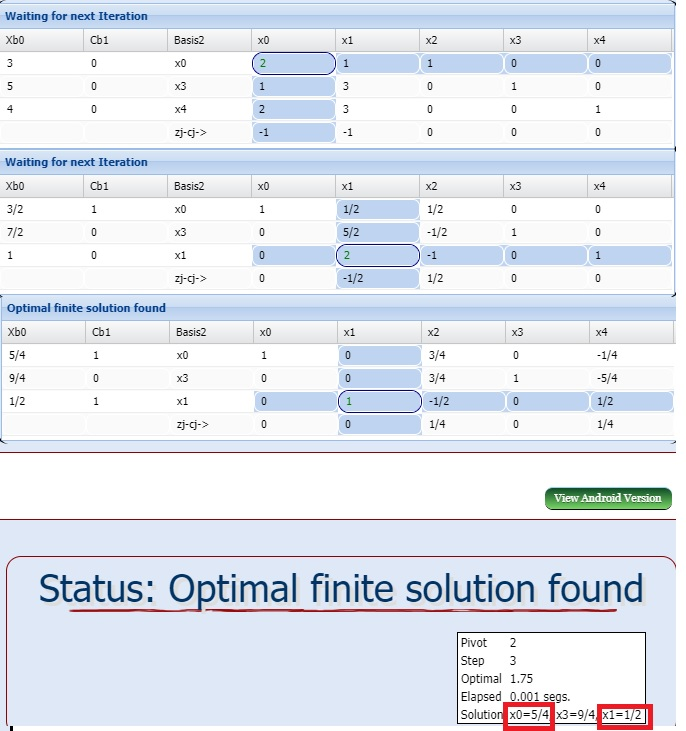
\includegraphics[scale=0.35]{8p18a}
    \caption{Primal Problem, and the optimal value is 1.75. \\ ..} \label{fig:}
    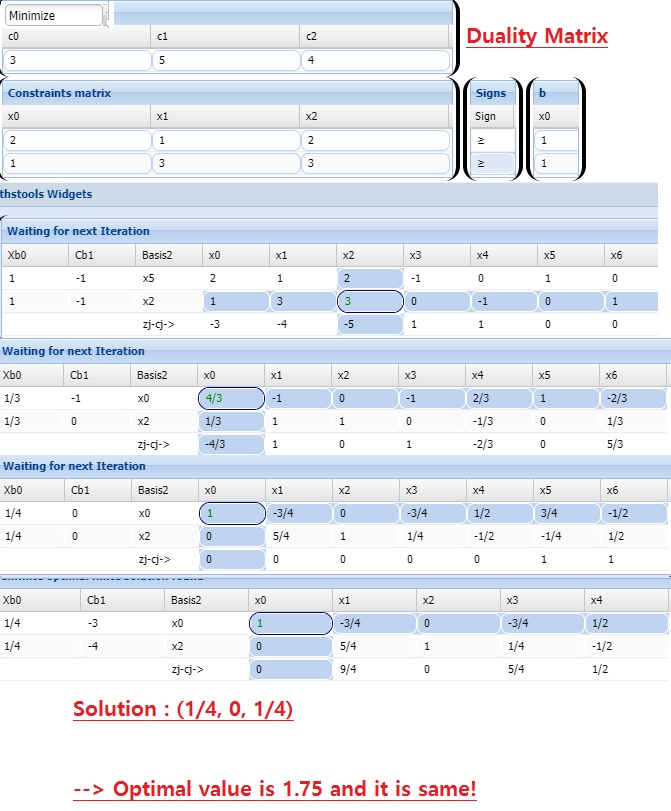
\includegraphics[scale=0.35]{8p18b}
    \caption{Dual Problem} \label{fig:label}
\end{center}
\end{figure}





















\end{enumerate}

\vspace{25mm}

\bibliography{ProbStat_probset}

\end{document}
